\documentclass[tikz]{standalone}
\usepackage{varwidth}
\usetikzlibrary{chains}
\begin{document}
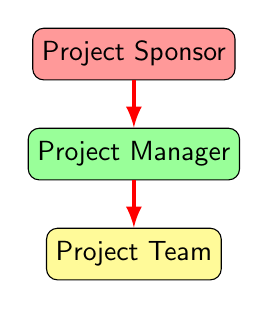
\begin{tikzpicture}[
    start chain=going below, node distance=6mm,
    every join/.style={->,>=latex, red, ultra thick},
    mynode/.style={
        rounded corners, draw, font=\sffamily,
        on chain, join,
        execute at begin node={\begin{varwidth}{5cm}\centering},
        execute at end node={\end{varwidth}}
    }
]
\foreach \mystep/\myexpl/\mycol in 
    {Project Sponsor//red!40,
    Project Manager//green!40,
    Project Team//yellow!40%
    }
    \node[mynode,fill=\mycol] {\strut\mystep\\\footnotesize\myexpl};
\end{tikzpicture}
\end{document}